\documentclass{standalone}
\usepackage{tikz}
\begin{document}
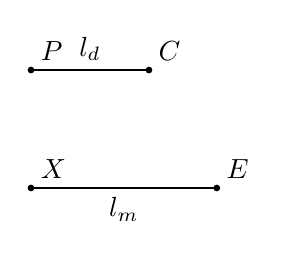
\begin{tikzpicture}[scale=0.5]
  \filldraw (0.0, 0.0) circle (2pt) node[above right] {$X$};
  \filldraw (4.7187, 0.0) circle (2pt) node[above right] {$E$};
  \filldraw (0.0, 2.9958) circle (2pt) node[above right] {$P$};
  \filldraw (2.9958, 2.9958) circle (2pt) node[above right] {$C$};
  \draw (0.0, 0.0) -- (4.7187, 0.0) node[midway, below] {$l_m$};
  \draw (0.0, 2.9958) -- (2.9958, 2.9958) node[midway, above] {$l_d$};
\end{tikzpicture}
\end{document}